\chapter{Introducción}
\section{Justificación}
    \par
    La cerveza es una bebida alcohólica no destilada de sabor amargo, fabricada a base de agua, cereales (principalmente cebada malteada), lúpulo y levadura.
    \par
    Las primeras cervezas, datadas alrededor del año 9000 A.C., fueron producto de una combinación de ciertos accidentes en el almacenado de granos y en la elaboración de pan. Con el avance del tiempo la receta de la cerveza se fue construyendo mediante ensayo y error de las técnicas utilizadas para elaborarla, perfeccionándose hacia finales del siglo XV.
    \par
    La cerveza artesanal tiene su origen a finales de 1970 en el Reino Unido, siendo esta utilizada para denotar pequeñas cervecerías o microcervecerías que se enfocaban en la producción tradicional. “Aunque el término microcervecería fue utilizado para describir el tamaño de las cervecerías, gradualmente pasó a reflejar una actitud y un enfoque alternativo a la flexibilidad en la producción de cerveza, adaptabilidad y atención al cliente” (Calvillo, E., 2017). En el año 2017 fue incorporado al Código Alimentario Argentino (Ley 18284, 2017, art. 1082 bis) la definición de cerveza de elaboración artesanal como “ … aquella que no utilice en su producción aditivos alimentarios... se encuentre adicionada únicamente con ingredientes naturales… y cuya elaboración sea de manera manual o semiautomática…”
    \par
    En la actualidad, las microcervecerías han adoptado una estrategia de mercadotecnia diferente a la de compañías de cerveza industrial, ofreciendo productos que compiten según su calidad y diversidad, en lugar de precios bajos y publicidad. En este sentido, se ha  impulsado una tendencia mundial al aumento del consumo y producción de cerveza artesanal, (Calvillo, E., 2017). En Argentina esta situación es reflejada en índices productivos, según Cuculiansky (2017) “Fuentes del sector estiman que el crecimiento es del 30\% anual y ya ostenta entre el 1,5\% y 2\% de la industria cervecera”. La misma promueve a un mayor número de productores cerveceros a iniciarse en la cocción, de acuerdo a Aizen (2017): “Hay unos mil productores de cerveza artesanal… de todo tipo: familiares, amigos, empresas medianas y de tamaño respetable también… ”. Con este esquema productivo y una gran alza de consumo, consecuencia del creciente número de bares de cerveza artesanal, se observa una marcada insatisfacción de la demanda, léase Ríos (2016).
    \par
    La inserción en este mercado depende de la estrategia de venta utilizada, apoyándose en la diversidad de estilos y calidad de las cervezas. Bajo este esquema, cada productor distingue sus productos en función de la variedad de tipos que ofrece, cada uno definido por un estilo y una receta con su sello personal. Esta impronta se define a partir de su criterio en la experimentación de recetas, la virtud de los insumos que utiliza, y la precisión y el control a lo largo del proceso de elaboración.
    \par
    El proceso de producción de cerveza, (en la jerga cocción), según algunos autores (Nachel, 2008, p.101; DOG Brewery, 2015, p.7; American HomeBrewers Association, 2018; Novozymes Co., 2013, p.2; entre otros), consta básicamente de siete etapas ordenadas en forma secuencial (Figura \ref{ProcFab}): maceración, recirculado, cocción, enfriamiento, fermentación, maduración, filtración. El mismo se resume muy brevemente de la siguiente manera: Se comienza por la maceración, que es un preparado de agua caliente y granos molidos de cebada malteada, cuya función es la de transformar en azúcares las cadenas de almidón presente en los granos; seguido a esto por un proceso de cocción, donde se hierve y esteriliza la solución (mosto) y se le incorpora el lúpulo, una hierba que aporta al mosto aroma y sabor. En las etapas finales, se produce alcohol a partir de la incorporación de levadura que consume el azúcar fermentable del preparado. Luego se filtra para remover sedimentos y finalmente se envasa.
    \par
    \begin{figure}[h]
		\centerline{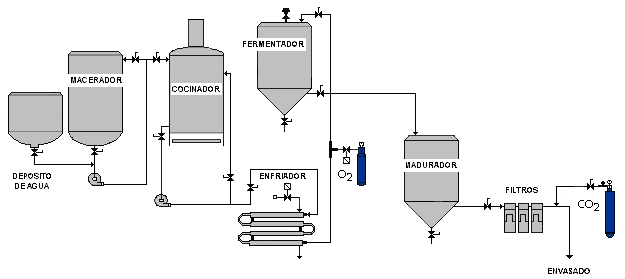
\includegraphics[scale=0.7]{procDeFab.jpg}}
		\caption{Proceso productivo para elaboración de cerveza en 7 etapas: maceración, recirculado, cocción, enfriamiento, fermentación, maduración, filtración}
	    \label{ProcFab}
	\end{figure}
	\par
	El Macerado es el proceso que reviste interés en este proyecto, según Palmer (2006) se define como “El proceso de remojado en agua caliente que promueve (provoca, fomenta) la descomposición enzimática de la molienda en azúcares solubles y fermentables“. Y, como explica Papazian (2003) “El proceso es continuado durante un período de tiempo con ajustes controlados de las temperaturas y pH que activa diferentes enzimas para descomponer los almidones solubles y las proteínas”.
	\par
    \begin{table}[ht]
        \begin{tabular}{|l|c|c|l|}
        \hline
            \multicolumn{1}{|l|}{Enzima} & \begin{tabular}[c]{@{}c@{}}Rango óptimo de\\ temperatura\end{tabular} & \begin{tabular}[|l|]{@{}c@{}}Rango de pH\\ de trabajo\end{tabular} & \multicolumn{1}{c|}{Función} \\ \hline \hline
            \multicolumn{1}{|l|}{Fitasa} & 30C - 52C & 5.0 - 5.5 & Baja el pH del mash\\\hline
            \multicolumn{1}{|l|}{Debranching} & 35C - 45C & 5.0 - 5.8 & Solubilización de almidones \\\hline
            \multicolumn{1}{|l|}{Beta Glucanasa} & 35C - 45C & 4.5 - 5.5 &\begin{tabular}[l]{@{}l@{}}Mejora la disolución de residuos\\ gomosos.\end{tabular}  \\\hline
            \multicolumn{1}{|l|}{Peptidasa} & 45C - 55C & 4.6 - 5.3 & Produce Free Amino Nitrogen \\\hline
            \multicolumn{1}{|l|}{Proteasa} & 45C - 55C & 4.6 - 5.3 &\begin{tabular}[l]{@{}l@{}}Reduce a partes pequeñas a las\\ grandes proteínas.\end{tabular}  \\\hline
            \multicolumn{1}{|l|}{Beta Amilasa} & 55C - 65.5C & 5.0 - 5.5 & Produce Maltosa \\\hline
            \multicolumn{1}{|l|}{Alpha Amilasa} & 67.8C - 72C & 5.3 - 5.7 & \begin{tabular}[l]{@{}l@{}}Produce Variedad de azúcares,\\ incluyendo maltosa.\end{tabular}\\ \hline
        \end{tabular}
        \caption{Rango de desempeño óptimo de las enzimas}
        \label{tablaEnzimas}
    \end{table}
    \par
    En la conformación de los granos aproximadamente el 80\% de los mismos es almidón o extracto que se puede transformar por descomposición enzimática para formar parte del mosto y el restante 20\% queda como desecho o bagazo que debe ser filtrado. El porcentaje de la materia prima utilizada en una maceración que queda conformando el mosto se conoce como rendimiento del grano que usualmente tiene valores dentro del rango 60\%-80\%. Para determinar el rendimiento se tiene que relacionar la densidad del mosto con el volumen de agua y el peso de los granos utilizados. Dicho valor al concluir la maceración (cálculo de rendimiento de la maceración) puede ser estimado utilizando valores estipulados de rendimiento según el tipo de grano involucrado, la temperatura de maceración y el tiempo que se prolongó dicho proceso.
    \par
    Existen distintas variaciones del proceso, si se utiliza durante todo el procedimiento un solo intervalo para ambas variables (temperatura y pH) se conoce como maceración simple, en cambio, cuando se utilizan distintos intervalos para una u otra variable se la conoce como maceración compleja. Esta última, la menos utilizada, permite utilizar granos no malteados con los que se pueden lograr diferentes productos, requiriendo mayor supervisión e intervención del productor durante el proceso.
    \par
    El control del proceso, en especial con procedimientos de macerado complejos, reviste una serie de dificultades desafiantes que desde una primera instancia no son evidentes. La evolución de la temperatura durante el proceso difiere según el clima y las características del equipo en cuanto a pérdida de calor, de la misma forma la evolución del pH condicionado por el grano que se utilice y la temperatura, activará diferentes enzimas que pueden afectar este valor. Todas estas variables esquivas de controlar, influyen en mayor o menor medida en diferentes procesos enzimáticos deviniendo en una muy vasta variedad de resultados. De esta manera, la ausente o reducida aplicación de correctos controles puede devenir en efectos indeseados como: escasa cantidad de azúcares convertidos debido a maceraciones apresuradas (de duración insuficiente) o a desvíos de temperatura y pH; aumento indeseable de la densidad de la mezcla debido a sobre-rendimiento de la malta o incorrectos valores de temperatura y tiempo; pH fuera de intervalos o alta temperatura produce inactivación de enzimas, no realizándose de esta manera los procesos químicos inherentes a esta etapa; incorrectas intervenciones en el proceso, producto de medidas de temperatura no representativas de todo el volumen debido a la variabilidad de las mismas en distintos puntos del macerador. Conflictos como los mencionados, entre otros, pueden resultar en producciones inconsistentes y, en casos extremos, pérdida de la producción.
    \par
    En la aplicación práctica, la realización de cálculos de rendimiento puede realizarse, como ya se mencionó, sobre una base teórica para la cual los valores de rendimiento de cada malta se encuentran tabulados, siendo estos datos valores esperados. Sin embargo, se presenta un gran desfasaje entre los cálculos teóricos y el rendimiento real, esto es consecuencia de la calidad de los insumos, las características del equipo y los elementos usados para medir. Por esto, el productor utiliza el cálculo de rendimiento teórico solo para obtener una idea aproximada de los insumos necesarios para cumplir con los objetivos que se propone en la receta a realizar. Otorgando confianza al cálculo y basándose sobre este, deviene la posibilidad de sub o sobre rendimientos de la malta, interfiriendo así en la receta e incluso en el costo final del producto (fueron agregados más insumos de los necesarios).
    

\section{Estado del arte}
    \par
    Las herramientas existentes realizan un monitoreo de todo el proceso de fabricación siendo las más reconocidas Brew-o-matic\textsuperscript{®}, BeerSmith\textsuperscript{®} y BrewersFriend\textsuperscript{®}. Algunas de estas herramientas de software presentan integraciones con productos de hardware para realización de medidas mediante sensores, pero solo para la etapa de fermentación, siendo Tilt® el paquete de sensores más utilizado. Estas requieren, en forma indistinta, el ingreso manual de los datos o variables intervinientes en forma muy detallada (tipo y marca de la malta, pH y concentración de sedimento del agua, temperaturas, tiempos, etc) para la realización de estimaciones de variables de control (densidad, volumen, etc), donde se utilizan heurísticas, ecuaciones, y características teóricas de los insumos, para luego ser utilizadas al concluir cada etapa, de forma de verificar que el proceso se comporta según lo esperado. Como se mencionó antes, las características teóricas producen resultados que difieren de los reales, por tanto estas herramientas resultan poco efectivas para el control de los procesos. Además, ninguna profundiza el proceso de maceración, solo ofreciendo el cálculo de rendimiento y de insumos en base teórica y para infusiones simples.

\section{Objetivos}
\label{secccionObjetivos}
    \par
    A continuación se presentan los objetivos definidos, en forma previa, para el desarrollo de este proyecto.
    \par
    Se propone desarrollar un prototipo de hardware y software para asistir al productor de cerveza artesanal en el proceso de maceración a través de planificación de procesos, monitoreo de variables mediante sensores, estimación de variables de control y análisis intensivo de variables intervinientes y sus relaciones según corresponda.
    \par
    Esta herramienta brinda al productor facilidad para realizar el seguimiento de la evolución del proceso, permitiendo identificar momentos apropiados donde realizar acciones correctivas, evitando consecuencias inalterables. Comportándose las variables (pH y temperatura) según lo esperado en los distintos períodos de la maceración, se evitan resultados disímiles entre diferentes maceraciones y se optimiza el rendimiento de la malta a través del control puntual de las actividades enzimáticas, derivando en una disminución de insumos y costos.
    \par
    La utilización de múltiples de sensores beneficia en la obtención de medidas más representativas de todo el volumen del macerador, aumentando la fiabilidad de las mediciones y los cálculos que se realicen a partir de ellas. De forma adicional, la ubicación fija de cada sensor permitirá la obtención de datos representativos de cada sector. De manera consecuente, beneficiará en la identificación de sectores de mayor pérdida de calor brindando una facilidad para la mejora de la aislación térmica del equipo.
    \par
    Para el uso de maceraciones complejas el proyecto cobra crítica importancia. Los estilos que involucran este tipo de maceración son, por lo general, esquivos a los cerveceros dada la dificultad para realizar el monitoreo y control de las variables intervinientes. Con el uso de esta herramienta se simplifica esta tarea, deviniendo en la posibilidad de realizar cocciones de recetas con poca presencia en el mercado. Adicionalmente la herramienta facilitará la planificación del proceso, y alertará al productor en los momentos exactos que se requiere su intervención.


    \subsection{Objetivos generales}
    \
        \par
        Desarrollar un prototipo de hardware y software para asistir al productor de cerveza artesanal en la planificación, seguimiento y evaluación del proceso maceración. 
    \subsection{Objetivos específicos}
        \begin{itemize}
            \item Analizar, diseñar y construir un sistema electrónico para la medición mediante sensores de las variables intervinientes en el proceso de maceración.
            
            \item Desarrollar una aplicación móvil que brinde funcionalidades que faciliten la planificación, seguimiento y evaluación del proceso de maceración.
            
            \item Analizar, desarrollar, aplicar y utilizar una interfaz como medio de comunicación entre el sistema electrónico y la aplicación móvil.
            
            \item Ensamblar y validar el prototipo como una construcción del sistema electrónico, la aplicación móvil y la interfaz.
        \end{itemize}
 
 
 
\section{Alcance}
    \par
    En este apartado se presenta el alcance del proyecto definido previo a su desarrollo. El cual incorpora, las inclusiones, exclusiones y supuestos que fueron considerados.
    \par
    Se desarrollará un prototipo de hardware y software compuesto por un sistema electrónico y una aplicación móvil. El primero estará formado por un conjunto de sensores ubicados en diferentes puntos que medirán y un controlador que transmitirá a través de la interfaz los valores de temperatura y pH del preparado. La segunda se encargará de brindar las funciones de planeamiento de procesos de maceración, simples y complejos, incorporando estimación de variables de control, configuración de estrategias de obtención, monitoreo y notificación de desvíos de medidas, registro de histórico de procesos, visualización gráfica, análisis estadístico y comparativo de la evolución temporal de variables intervinientes en diferentes maceraciones a partir de muestras puntuales, medidas representativas o valores ingresados.
    \par
    El sistema será desarrollado para un usuario con conocimientos teóricos suficientes que pueda entender y relacionar la información presentada, y reaccionar en consecuencia si el proceso lo requiere. El mismo, será responsable del ingreso manual de datos de insumos, medidas de densidad, y comienzo y fin del proceso en la aplicación móvil.
    \par
    El desarrollo no proveerá un sistema automatizado de macerado ni una planificación, seguimiento y evaluación del proceso, sino que proveerá datos útiles y fidedignos a través de sus funcionalidades para asistir en dichas actividades. Será un prototipo funcional que cumpla las características previamente mencionadas sin alcanzar la etapa de implementación.
    \par
    Se supone que el dispositivo móvil cuenta con los servicios Wi-Fi y Bluetooth funcionando en forma correcta y utiliza una versión actual del sistema operativo o de no más de un año de antigüedad en relación a la fecha de este desarrollo. En caso de utilizar conexión Wi-Fi para la interfaz, se deberá disponer de un dispositivo de red Router para el establecimiento de una red local y se configurarán los parámetros de red del sistema electrónico en forma manual.
    \par
    La precisión de los valores medidos difiere según la calidad de los sensores. Como se propone el desarrollo de un prototipo, los mismos pueden no ser exactos y no se realizará un análisis en profundidad en relación a este nivel de precisión. 
    \par
    Se deja para un futuro desarrollo, la posibilidad de supervisar múltiples maceradores simultáneamente. 
 
        
\section{Metodología}

    \par
    En este apartado se presenta la metodología seleccionada previo al desarrollo de este proyecto.
    \par La metodología seleccionada para este proyecto es la de ciclo de vida en cascada enmarcando el desarrollo completo del sistema. En el mismo, cada proceso es secuencial y la finalización de uno de ellos es el punto de inicio del siguiente.
    
    \par Al finalizar cada etapa se presentará un hito, que será el resultado de la etapa, el cual estará sujeto a determinados criterios de aceptación. En cada etapa, el director del proyecto será quien juzgue si los resultados obtenidos satisfacen estos criterios.


    \paragraph{Etapas:}
        \begin{enumerate}
            \item Análisis temático y de requerimientos:
                \par En la etapa inicial se realizará una investigación bibliográfica, enfocada en el estudio del procedimiento de fabricación de cerveza artesanal, con especial atención en los procesos y subprocesos del macerado. Se redactará en forma adicional un análisis de requerimientos para el proyecto. Al finalizar esta etapa se documentará el Análisis temático que contendrá las bases teóricas que sustentan este proyecto.
                \par \textit{Hito 1: Adquisición de conocimientos necesarios.}
                
            \item Análisis, diseño y desarrollo del componente Hardware:
                \par Se llevará a cabo una investigación y análisis de potenciales soluciones para el abordaje del hardware, luego se  documentará esta investigación y se justificará la elección de la solución. Luego, se realizará un aprendizaje de desarrollo de la tecnología utilizada en la solución, para en forma consecuente, realizar el diseño y desarrollo de este sistema.
                \par \textit{Hito 2: Sistema electrónico desarrollado.} 
                
            \item Análisis, diseño y desarrollo del componente Software:
                \par En esta etapa, se realizará una investigación y análisis de potenciales tecnologías móviles a utilizar que serán documentadas junto a la elección de mayor conveniencia para esta etapa. A continuación, se realizará un aprendizaje de desarrollo de aplicaciones en esta tecnología, para en forma consecuente, producir el diseño y desarrollo de la aplicación.
                \par \textit{Hito 3: Aplicación móvil desarrollada.}
                
            \item Análisis, diseño y desarrollo de la Interfaz Hardware - Software:
                \par Se entiende la interfaz como un espacio,  lugar donde se desarrolla la interacción y el intercambio entre dos sistemas. Disponiendo del sistema de hardware y la aplicación móvil, se realizará una investigación y análisis de posibles alternativas, procediendo a continuación con el desarrollo de la misma.
                \par \textit{Hito 4: Interfaz desarrollada.}
                
            \item Integración y ciclo de pruebas:
                \par Se realizará la integración de los desarrollos y un ciclo de pruebas de campo para corroborar el correcto funcionamiento del sistema. Concretando con la redacción del informe final del proyecto.
                \par \textit{Hito 5: Proyecto Finalizado.}

        \end{enumerate}
